\section{方法}


\subsection{近接2粒子ホログラムの検証実験}
式(\ref{th:stripepattern})に示した関係が正しく成り立ち,この関係によって縞パターンから粒子組の近接状態を正しく決定できることを実験によって検証する.実験装置の概念図をFig. \ref{fig:stripePatternExperiment}に示す.本実験では,直径\SI{250}{\um}の円形ドットが印刷されたガラスプレートを2枚用いて粒子間距離 $(\Delta \xi, \Delta \eta )$ を操作し,それぞれの粒子ホログラムのスペクトル分布から粒子間距離を推定する.Table \ref{table:stripePatternExperiment}に実験条件を示す.$y$ 軸方向の粒子間距離は常に $\Delta \eta = \SI{0}{\um}$ とし,$x$軸方向の粒子間距離 $\Delta \xi$ をマイクロメータで操作する.また,本実験では粒子間の$z$軸方向距離が\num{0}であると仮定する.そのために,接着した2枚のガラスプレートの間には,屈折率 \num{1.51253} の屈折率マッチングオイル (Immersion Oil Type A, Cargille) を充填し,2枚のガラスプレート間で回折が起こらないようにする. 

\begin{figure}[H]
    \centering
    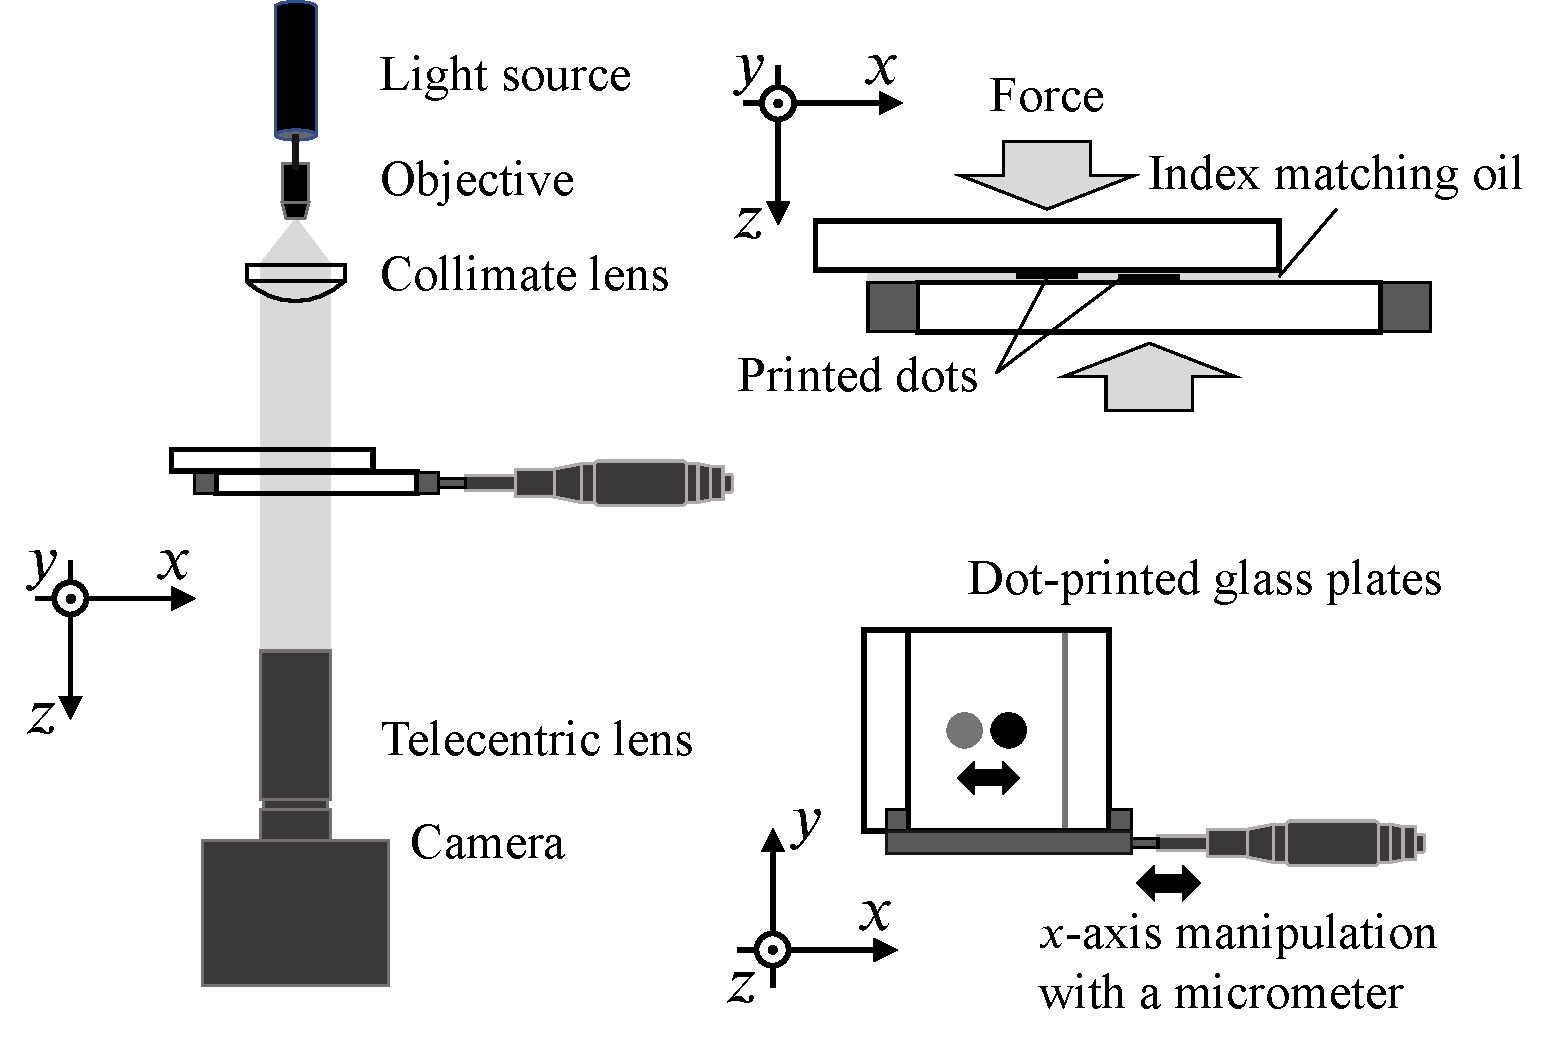
\includegraphics[width=0.8\linewidth]{./Figure/3_Methods/stripe_pattern_experiment.pdf}
    \caption{Schematic diagram of experimental setup. The $x$-axis distance between dots is varied by manipulating one of the two glass plates with dots printed on them with a micrometer. The printing surfaces of the glass plates are fixed facing each other. The space between the plates is filled with refractive index matching oil (Immersion Oil Type A, Cargille, Refractive Index: 1.51253) to prevent diffraction caused by the gap between them.}
    \label{fig:stripePatternExperiment}
\end{figure}

\begin{table}[H]
    \centering
    \caption{Experimental conditions to verify the relationship between the stripe pattern formed on the spectral distribution of particle holograms and the distance between particles.}
    \label{table:stripePatternExperiment}
    \begin{tabular}{lll}
    Quantity                               & Value                                             & Unit     \\ \hline \hline
    Dot diameter $2a$                      & 250                                               & \si{\um} \\ \hline
    Dot distance in $x$-axis $\Delta \xi$  & Every 10 from 0 to 500, every 50 from 500 to 1000 & \si{\um} \\ \hline
    Dot distance in $y$-axis $\Delta \eta$ & 0                                                 & \si{\um} \\ \hline 
    Recorded wavelength $\lambda$          & 632.8                                             & \si{\nm} \\ \hline
    Propagated distance $z_0$              & 250                                               & \si{\mm} \\ \hline
    Pixel pitch of hologram $\Delta x$     & 10                                                & \si{\um}
    \end{tabular}
\end{table}


\subsection{水滴近接検出モデルの学習と推論}\label{sec:EffNetV2}
この節では,\ref{sec:twoParticleHologramFeature}節で示した近接粒子ホログラムのスペクトル分布上に現れる縞パターンを検出するための畳み込みニューラルネットワークモデルを構築・学習および評価するための方法について示す.

\subsubsection{学習データ生成}
\ref{sec:in-lineHolography}節および\ref{sec:twoParticleHologramFeature}節で示したように,粒子ホログラムは数値生成が可能である.本論文ではモデル学習のために数値生成したホログラムデータを用いる.生成するデータの諸条件をTable \ref{table:trainingData}に示す.

\begin{table}[H]
    \centering
    \caption{Conditions for generating hologram data for model training.}
    \label{table:trainingData}
    \begin{tabular}{lll}
    Quantity & Value & Unit \\ \hline \hline
    Hologram image size & $\num{256} \times \num{256}$ & \si{pixel\squared} \\ \hline
    Pixel pitch & \num{10} & \si{\um} \\ \hline
    Mean particle diameter & \num{85} & \si{\um} \\ \hline 
    Standard deviation of particle diameter & \num{23} & \si{\um} \\ \hline
    Particle number & up to 3 in positive condition & - \\
    & up to 8 in negative condition & - \\ \hline
    Generated holograms & \num{1000000} for each condition & - \\ \hline
    Propagated distance & \num{220} to \num{270} & \si{\mm} \\ \hline
    Recorded wavelength & \num{632.8} & \si{\nm} \\ \hline
    \end{tabular}
\end{table}

記録されたホログラムのうち,接近粒子組を含むものを positive 条件,接近粒子組を含まないものを negative 条件として分類する.Positive ホログラムには,接近する2つの粒子と余分な1つの粒子を含む3つまでの粒子が記録される.Negative ホログラムには,接近する粒子組を含まない8つまでの粒子が記録される.すべてのホログラムは,人為的に配置される近接粒子組以外の粒子はすべて互いに離れて配置される.本論文におけるPositiveデータの近接距離しきい値は以下によって定める.
\begin{gather}
    \sqrt{\Delta \xi^2 + \Delta \eta^2} < \SI{200}{\um} \\
    |z_{pi}-z_{pj}| < \SI{6000}{\um} \\
\end{gather}
近接しきい値は,平面方向,奥行方向それぞれで粒子組の半径の和より大きければ原理的にはどの値であってもよいが,これらの値が小さいほど実際の時系列画像に対する推論では連続抽出フレーム数が小さくなる.水滴の相対速度が1フレームあたり\SI{20}{pixel}以上ある場合は水滴衝突に際する形状変化を観測することが難しいため,本実験ではこの値に設定する.また,平均粒径\SI{85}{\um}の粒子の伸び長さは式(\ref{th:elongationLength})より$n=1$として約\SI{5.7}{\mm}あるため,平面内距離条件を満たし,かつ奥行方向に\SI{6}{\mm}以内にある粒子組を近接粒子組とする.

以上の条件に従って生成したデータの例とそのスペクトル分布をFig. \ref{fig:trainingData}に示す.Positi
ve データのスペクトル分布には粒子近接に伴う縞パターンが現れており,Negative データのスペクトル分布には縞パターンは現れないことを確認できる.

数値生成したデータのみによる学習では,ノイズを含む実験データに対するモデルの推論性能が低下する可能性がある.そこで,後に実際に推論を行う実験データの背景ノイズを数値生成したデータに付与する.背景ノイズは,Table \ref{table:backgroundnoisecondition}に示す撮影条件で得た高速度画像を背景除去して得る時間列データから得る.ある背景ノイズデータの輝度値分布をFig. \ref{fig:backgroundnoise}に示す.

\begin{figure}[H]
    \centering
    \begin{subfigure}[t]{0.45\linewidth}
        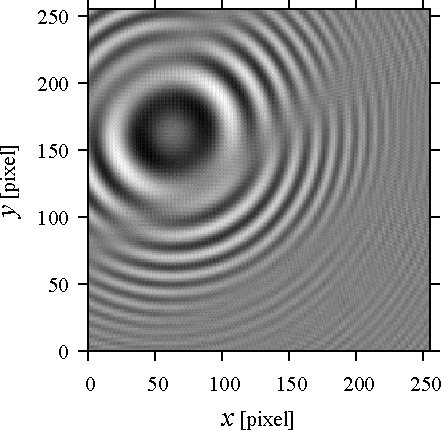
\includegraphics[width=\linewidth]{./Figure/3_Methods/close1.pdf}
        \caption{Positive hologram}
        \label{fig:trainingData:posiholo}
    \end{subfigure}
    \hfill
    \begin{subfigure}[t]{0.45\linewidth}
        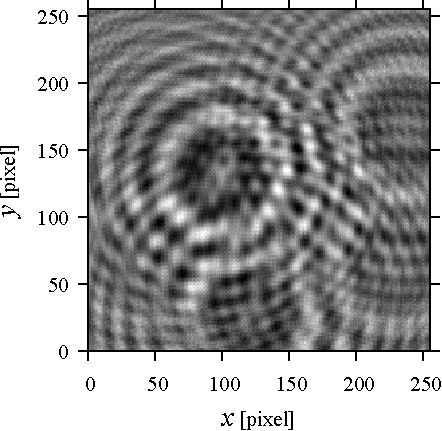
\includegraphics[width=\linewidth]{./Figure/3_Methods/far1.pdf}
        \caption{Negative hologram}
        \label{fig:trainingData:negaholo}
    \end{subfigure}

    \begin{subfigure}[t]{0.45\linewidth}
        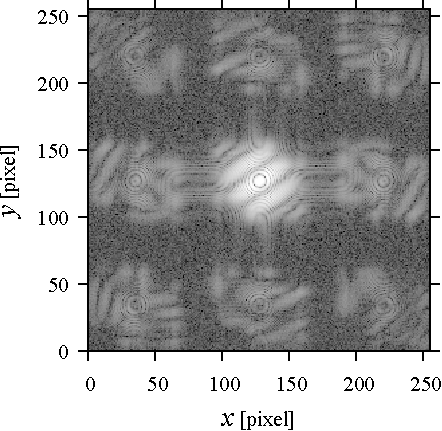
\includegraphics[width=\linewidth]{./Figure/3_Methods/fftclose1.pdf}
        \caption{Positive hologram spectrum}
        \label{fig:trainingData:posispec}
    \end{subfigure}
    \hfill
    \begin{subfigure}[t]{0.45\linewidth}
        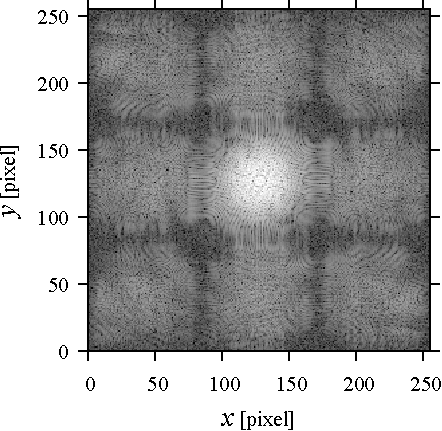
\includegraphics[width=\linewidth]{./Figure/3_Methods/fftfar1.pdf}
        \caption{Negative hologram spectrum}
        \label{fig:trainingData:negaspec}
    \end{subfigure}

    \caption{Example of generated holograms and their spectrum for training. Holograms are generated with the conditions shown in Table \ref{table:trainingData}, and the hologram spectrum is calculated by Fourier transform, logarithmically converted, and normalized. All data above are contrast-enhanced for visualization.} 
    \label{fig:trainingData}
\end{figure}



\begin{table}[H]
    \centering
    \caption{Conditions for generating background noise data.}
    \label{table:backgroundnoisecondition}
    \begin{tabular}{lll}
    Quantity & Value & Unit \\ \hline \hline
    Image size & $\num{256} \times \num{256}$ & \si{pixel\squared} \\ \hline
    Pixel pitch & \num{10} & \si{\um} \\ \hline
    Particle number & 0 & - \\ \hline
    Recorded wavelength & \num{632.8} & \si{\nm} \\ \hline
    \end{tabular}
\end{table}

\begin{figure}[H]
    \centering
    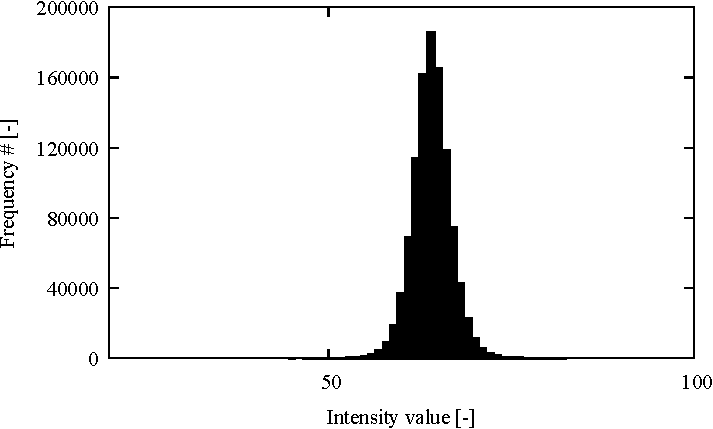
\includegraphics[width=0.8\linewidth]{./Figure/3_Methods/noisehistogram.pdf}
    \caption{Light intensity distribution of background noise data.}
    \label{fig:backgroundnoise}
\end{figure}

\subsubsection{モデル構築および学習}
この節では,Pytorch\cite{paszke2019}とPytorch Image Models (timm)\cite{rw2019timm}を用いてモデルを構築し,学習を行う方法について示す.Table \ref{table:EffNetV2-S}にEfficientNetV2-Sのモデル構成を示す\cite{tan2021}.また,Table \ref{table:EffNetV2-XL}に,EfficientNetV2-SのスケールモデルであるEfficientNetV2-XLのモデル構成を示す.2つのモデルは各Stageにおける層の数やチャネル数,Flatten層直前のMBConv層の有無などが異なるが,Flatten層への入力パラメータ数は1280で共通であり,同じ取扱いが可能である.図中 Conv2d は\ref{sec:convolutionalLayer}節で示した基本的な畳み込み層を示す.Skip connectionはResNet\cite{he2016}で示されたスキップ接続であり,畳み込み層出力を入力を足したものを層の出力とする.SEは Squeeze-and-Excitation \cite{hu2018} を示し,畳み込み層の各チャネルに重み付けを行うアテンション機構である.MBConv\cite{tan2019}やFused-MBConv\cite{tan2021}は,Expansion ratioによって増加させた畳み込み層のチャネル数を再びSEによってもとの次元に減少させてモデルの表現能力を向上させる.畳み込み層の出力はFlatten層で一次元ベクトル化され,2クラス分類を行う全結合層(FC)に入力される.全結合層は出力次元が100, 10, 2の3層からなり,前の2層でBatch Normalization\cite{ioffe2015}とReLU\cite{nair2010}を適用する.最終層はSigmoid関数を適用する.

本論文ではまずEfficientNetV2-Sモデルによって,これまでに局所特徴を示したホログラムのスペクトル分布を学習するモデルと,スペクトル分布ではなくホログラムから直接学習する2つのモデルを比較する.フーリエ変換は可逆変換であり,スペクトル分布上縞パターンの情報はホログラムフリンジにも含まれているため,モデルがホログラム画像から直接学習することが可能であれば前処理としてのフーリエ変換を省略することができ,計算コストを削減できる.ホログラム画像から直接モデルを学習できることを確認した後,よりパタメータが多く,EfficientNetV2-Sよりも特徴抽出能力が高いEfficientNetV2-XLモデルによって学習を行い,推論精度向上を図る.

\newpage
\begin{table}[H]
    \centering
    \caption{EfficientNetV2-S model architecture; this model architecture is the reference implementation by the authors of the paper and differs from the original implementation described in the paper. The original one has another Fused-MBConv layer between Stage 0 and 1.}
    \label{table:EffNetV2-S}
    \begin{tabular}{lllllll}
    Stage & Operator & Kernel size & Stride & Channels & Layers & Other option \\ \hline \hline
    0 & Conv2d & 3 & 1 & 24 & 2 & Skip connection \\ \hline
    1 & Fused-MBConv & 3 & 2 & 48 & 4 & Expansion ratio 4 \\ \hline
    2 & Fused-MBConv & 3 & 2 & 64 & 4 & Expansion ratio 4 \\ \hline
    3 & MBConv & 3 & 2 & 128 & 6 & Expansion ratio 4, \\ &&&&&& SE ratio 0.25  \\ \hline
    4 & MBConv & 3 & 1 & 160 & 9 & Expansion ratio 6, \\ &&&&&& SE ratio 0.25  \\ \hline
    5 & MBConv & 3 & 2 & 256 & 15 & Expansion ratio 6, \\ &&&&&& SE ratio 0.25  \\ \hline
    6 & Flatten & - & - & 1280 & 1 & - \\ \hline
    7 & FC & - & - & 2 & 3 & - \\ \hline
    \end{tabular}
\end{table}

\begin{table}[H]
    \centering
    \caption{EfficientNetV2-XL model architecture; this model is the scaled-up variant of EfficientNetV2-S. The input parameters of the Flatten layer are 1280, consistent with the small variant.}
    \label{table:EffNetV2-XL}
    \begin{tabular}{lllllll}
    Stage & Operator & Kernel size & Stride & Channels & Layers & Other option \\ \hline \hline
    0 & Conv2d & 3 & 1 & 32 & 4 & Skip connection \\ \hline
    1 & Fused-MBConv & 3 & 2 & 64 & 8 & Expansion ratio 4 \\ \hline
    2 & Fused-MBConv & 3 & 2 & 96 & 8 & Expansion ratio 4 \\ \hline
    3 & MBConv & 3 & 2 & 192 & 16 & Expansion ratio 4, \\ &&&&&& SE ratio 0.25  \\ \hline
    4 & MBConv & 3 & 1 & 256 & 24 & Expansion ratio 6, \\ &&&&&& SE ratio 0.25  \\ \hline
    5 & MBConv & 3 & 2 & 512 & 32 & Expansion ratio 6, \\ &&&&&& SE ratio 0.25  \\ \hline
    6 & MBConv & 3 & 1 & 640 & 8 & Expansion ratio 6, \\ &&&&&& SE ratio 0.25  \\ \hline
    7 & Flatten & - & - & 1280 & 1 & - \\ \hline
    8 & FC & - & - & 2 & 3 & - \\ \hline
    \end{tabular}
\end{table}
\newpage

本研究で用いるEfficientNetV2モデルはImageNet-21k\cite{krizhevsky2012}で事前学習したものを用いるため,モデルのFlatten層までの畳み込み層は転移学習ではパラメータを更新しない.ImageNet-21kにはホログラム画像は含まれていないが,この事前学習によって画像認識モデルの畳み込み層は画像特徴を抽出する能力を持つ.抽出された特徴マップから近接粒子の有無を判定するためにランダムな値で初期化した全結合層を接続しており,この層のパラメータを学習することでモデルは近接粒子を検出できるようになる.

モデルの損失関数は交差エントロピー誤差\cite{bishop2006}を,最適化手法はAdam\cite{kingma2015}を用いる.学習率は初期値\num{6e-5}で,学習率減衰は\num{0.7}を用いて,学習率減衰のタイミングは学習のエポック数が\num{3}の倍数のときに行う.この手法はPytorchでStepLRとして提供される.モデルの学習は,学習データのうち\num{5}\%を検証データとして用いる.学習はGPUを用いて行う.

\subsubsection{モデル評価}\label{sec:modelEvaluation}
学習したモデルの評価方法について示す.Table \ref{table:evalclass}に,モデルの推論結果と実際のラベルの組み合わせによって分類される分類クラスを示す.これらのラベルを用いて,モデルの評価指標としてAccuracy,Precision,Recallを以下に定義する.
\begin{align}
    Accuracy &= \frac{TP + TN}{TP + FP + FN + TN} \\
    Precision &= \frac{TP}{TP + FP} \\
    Recall &= \frac{TP}{TP + FN}
\end{align}
Accuracyは主にデータのPositive-Negative比が1に近い場合によく用いられる評価指標である.PrecisionはPositiveと予測したデータのうち,実際にPositiveであるデータの割合を示す.Recallは実際にPositiveであるデータのうち,Positiveと予測されたデータの割合を示す.PrecisionやRecallはデータのPositive-Negative比が1から大きく異なる場合にも用いることができる.これらの評価指標は,モデルの推論結果から予測ラベルをPositiveとするためのしきい値によって変化する.モデルは,データがPositiveである確度(Confidence)を0から1の実数で表現するため,この範囲の変化するしきい値に対してPrecision,Recallを計算し,しきい値で対応するこれらの値をPrecision-Recall図にプロットしたものをPrecision-Recall曲線と呼ぶ.Precision-Recall曲線の下の面積をAUC (Area Under Curve)と呼び,モデルの推論性能を示す指標として用いる\cite{saito2015}.
\begin{table}[H]
    \centering
    \caption{Predicted class by model inference and actual label.}
    \begin{tabular}{c|c | cc}
        \multicolumn{2}{l|}{\multirow{2}{*}{}}  & \multicolumn{2}{c}{Predicted label} \\ \cline{3-4}
        \multicolumn{2}{l|}{}                   & Positive         & Negative         \\ \hline 
        \multirow{2}{*}{True label} & Positive & TP               & FN               \\ \cline{2-4}
                                    & Negative & FP               & TN              
        \end{tabular}
    \label{table:evalclass}
\end{table}


\subsection{時系列水滴ホログラムの撮影実験}
\subsubsection{実験装置と記録条件}
\ref{sec:EffNetV2}節で構築したモデルを用いて,実験で撮影した時系列水滴ホログラムから近接水滴組を抽出する.この節では,時系列水滴ホログラムの記録方法について示す.実験で用いた水滴噴霧装置と光学系をFig. \ref{fig:dropletSpray}に示す.また,記録条件をTable \ref{table:dropletSprayCondition}に示す.本実験では,2つのネブライザ (EW-KA 30, Panasonic) から噴霧した水滴が衝突する領域を2台の高速度カメラ(FASTCAM Mini UX100 type 800K-M-16G, Photron)で撮影する.観測領域からカメラまでの光伝搬距離を変化させ2枚のホログラムを記録することで\ref{sec:phaseRetrieval}節で示した位相回復を行う.カメラに装着したテレセントリックレンズ(VS-LTC1-130/FS, VS Technology)によって平行光をイメージセンサに記録することができる.観測領域で一様等方性乱流を発生させる8つのファンは,すべて定格の\SI{12}{\V}で駆動する.本来は観測領域で適切に一様等方性乱流場が発生しているか検証する必要があるが,本論文ではその検証は行わず,将来の課題とする.

\begin{figure}[H]
    \centering
    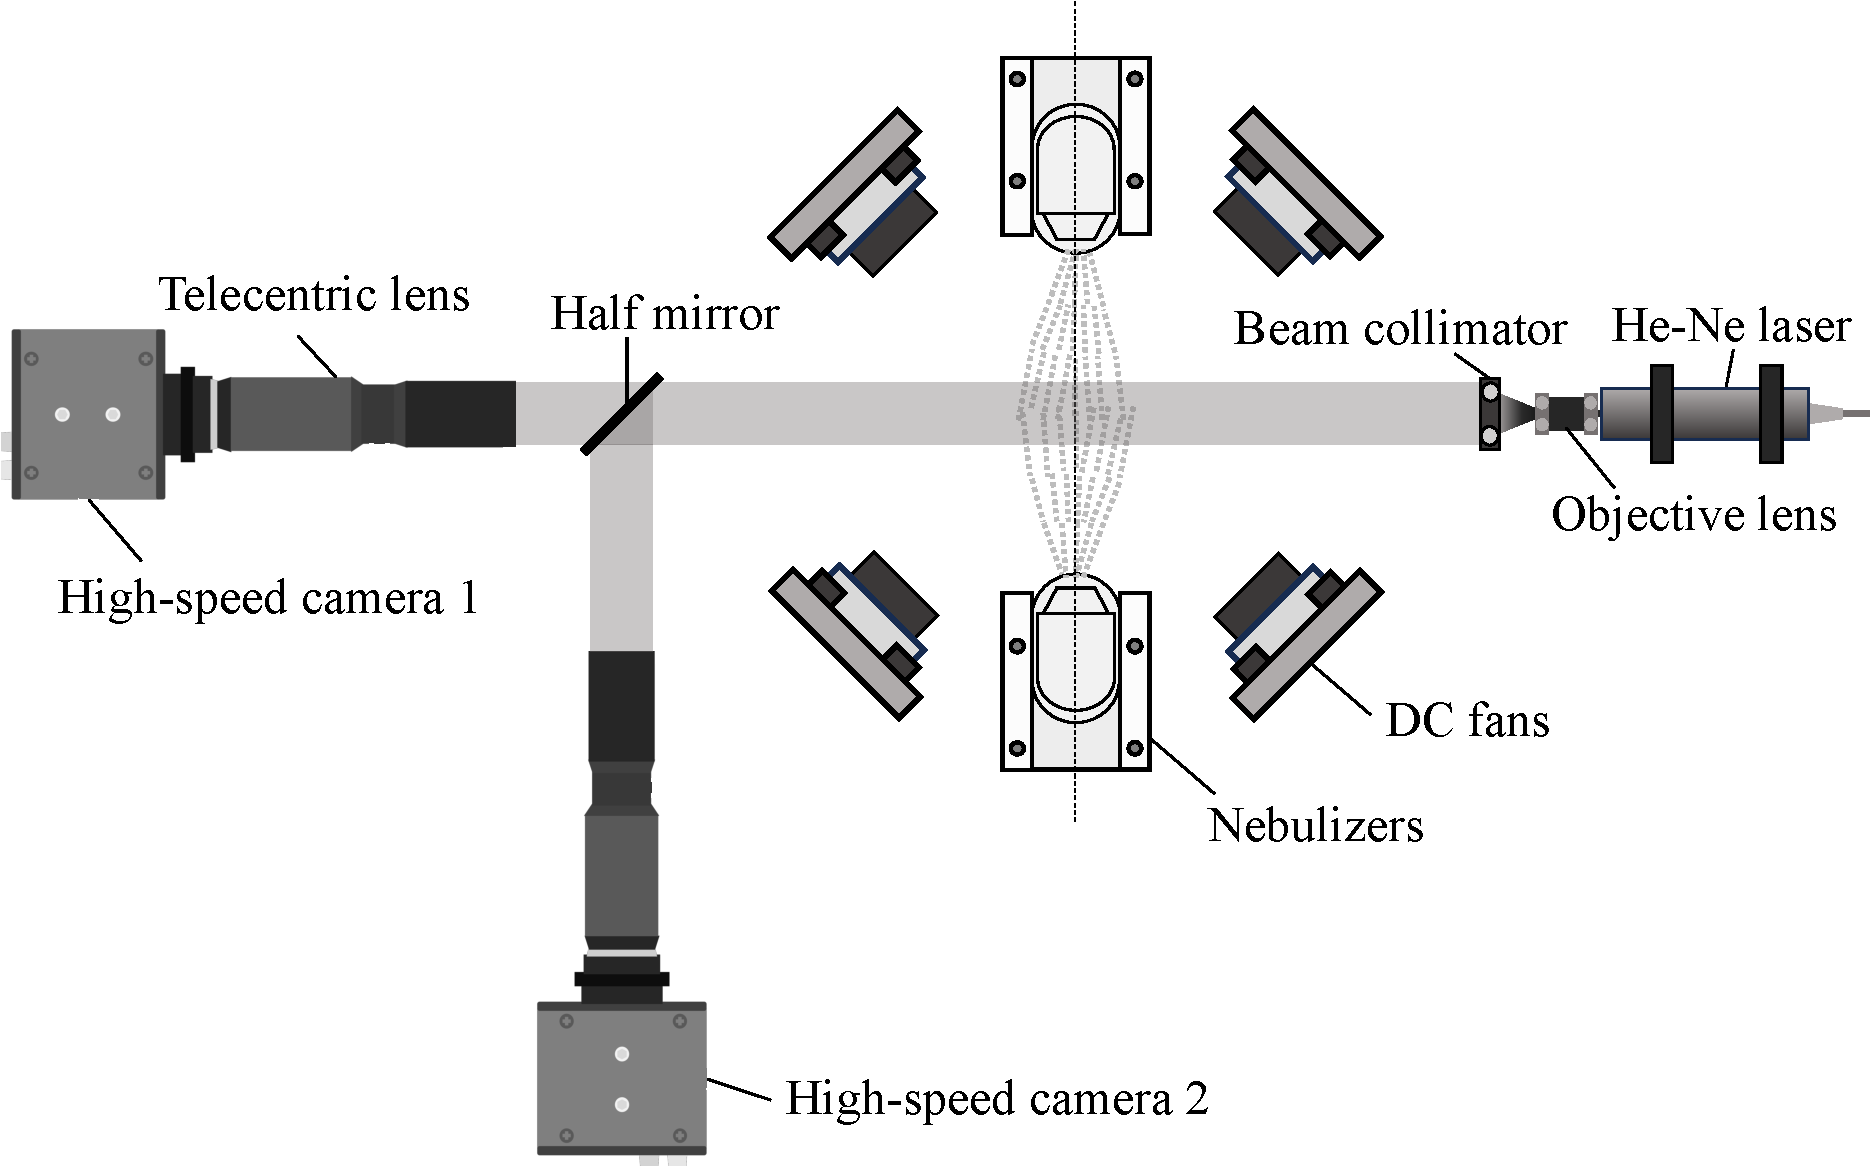
\includegraphics[width=0.8\linewidth]{./Figure/3_Methods/dropletspraysystem.pdf}
    \caption{Schematic diagram of droplet spray device and optical system; expanded and collimated He-Ne laser beam illuminates the droplet spray, and the holograms are recorded by two high-speed cameras with telecentric lenses. Eight DC fans are used to generate a uniformly isotropic turbulent field in the observation area.}
    \label{fig:dropletSpray}
\end{figure}

\begin{table}[H]
    \centering
    \caption{Conditions for recording holograms of droplet spray.}
    \label{table:dropletSprayCondition}
    \begin{tabular}{lll}
    Quantity & Value & Unit \\ \hline \hline
    Hologram image size & $\num{1024} \times \num{1024}$ & \si{pixel\squared} \\ \hline
    Pixel pitch & \num{10} & \si{\um} \\ \hline
    Recorded wavelength & \num{632.8} & \si{\nm} \\ \hline
    Propagated distance $z_1$ & \num{220} & \si{\mm} \\ \hline
    Propagated distance $\Delta z$ & \num{110} & \si{\mm} \\ \hline
    Exposure time & \num{250} & \si{\us} \\ \hline

    \end{tabular}
\end{table}

\subsubsection{2カメラの校正}
Fig. \ref{fig:dropletSpray}に示すシステムで撮影した2枚の同時ホログラムは,観測領域からの伝搬距離が異なるため異なるホログラフィックパターンを記録するが,位相回復ホログラフィによってカメラ1における位相分布を復元するためには2枚のホログラムが異なる$z$座標に対して等しい$x$-$y$平面を記録している必要がある.この節では,撮影した2枚のホログラムを校正する方法について示す.

カメラ画像校正にはバンドルアジャストメント\cite{okamoto2014}を用いる.本実験に際しては,直径\SI{70}{\um}のドットがランダムに印刷されたガラスプレートを2台のカメラで撮影し,それぞれをGabor再生して得た像からPIV\cite{willert1991}と等しいアルゴリズムで2カメラの回転・並進によるずれを計算する.コントラストを上げた2枚の再生画像と計算したベクトル場をFig. \ref{fig:beforebundle}に示す.
\begin{figure}[H]
    \centering
    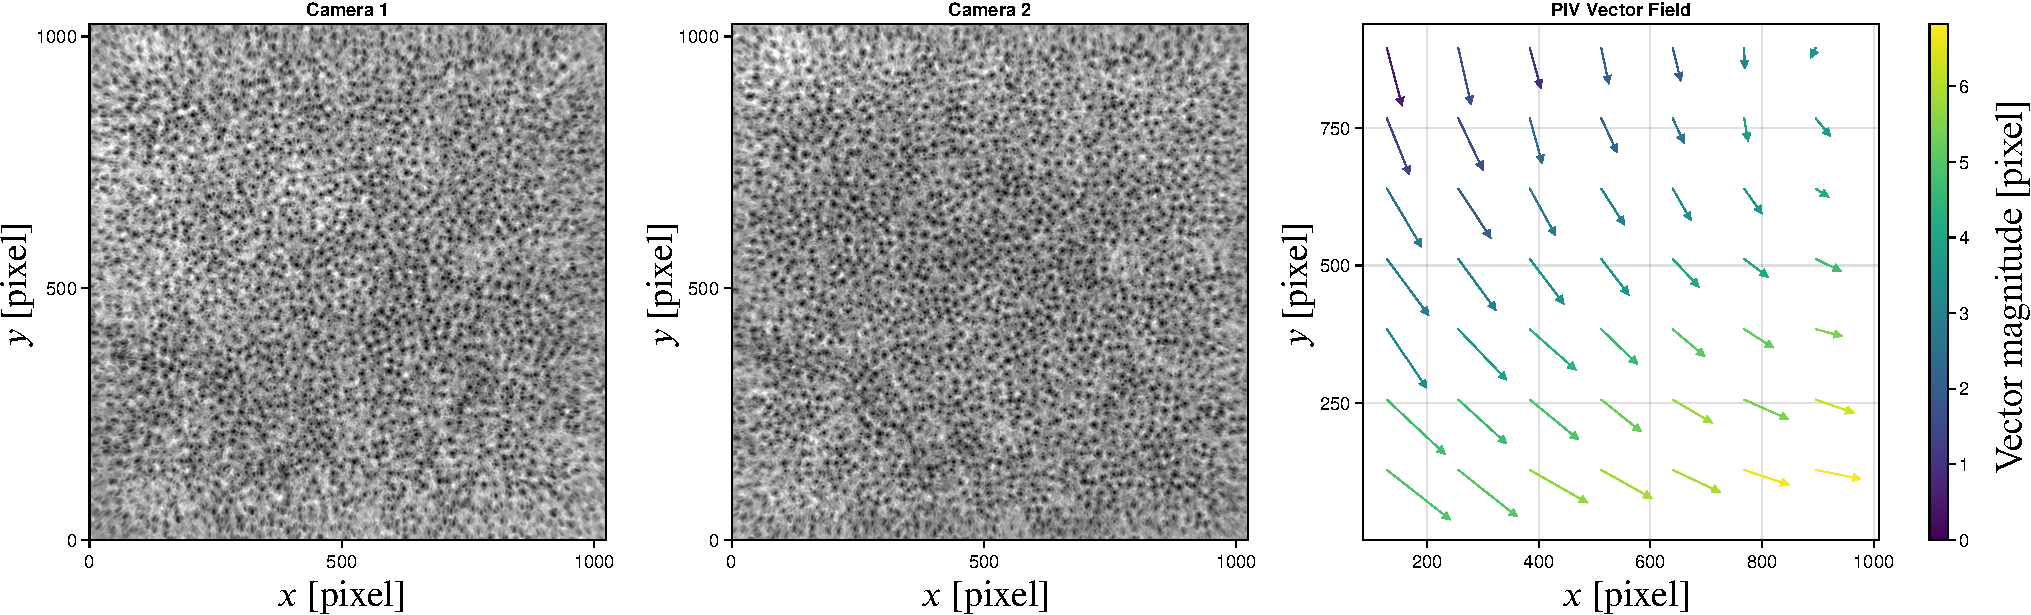
\includegraphics[width=0.98\linewidth]{./Figure/3_Methods/beforebundle.pdf}
    \caption{Reconstructed two random dot images with planer misalignment and the vector field calculated by PIV algorithm. Two images are contrast-enhanced for visualization.}
    \label{fig:beforebundle}
\end{figure}

取得したベクトル場は2枚の画像の平面内のずれを示すため,これを全域で0にするような画像変換$T$を実現すれば2枚の画像を校正できる.この画像変換$\bm{a}$は,カメラ1の座標を $(x_1,y_1)$,変換後のカメラ2の座標を $(x_2,y_2)$ とすると,以下のように表される.
\begin{equation}
    \left\{ 
    \begin{aligned}
        x_2 &= a_0 + a_1 x_1 + a_2 y_1 + a_3 x_1^2 + a_4 x_1 y_1 + a_5 y_1^2 \\
        y_2 &= a_6 + a_7 x_1 + a_8 y_1 + a_9 x_1^2 + a_{10} x_1 y_1 + a_{11} y_1^2
    \end{aligned}
    \right.
    \label{eq:bundle}
\end{equation}
理想の画像変換によって得る$(x_2,y_2)$と上記の画像変換によって得る$(x_2,y_2)$の差を最小化するようにパラメータ$a_i$に関する正規方程式を解く.実際にはパラメータ最適化はニュートン法を用いて行う.このようにして得られた画像変換をFig. \ref{fig:afterbundle}に示す.
\begin{figure}[H]
    \centering
    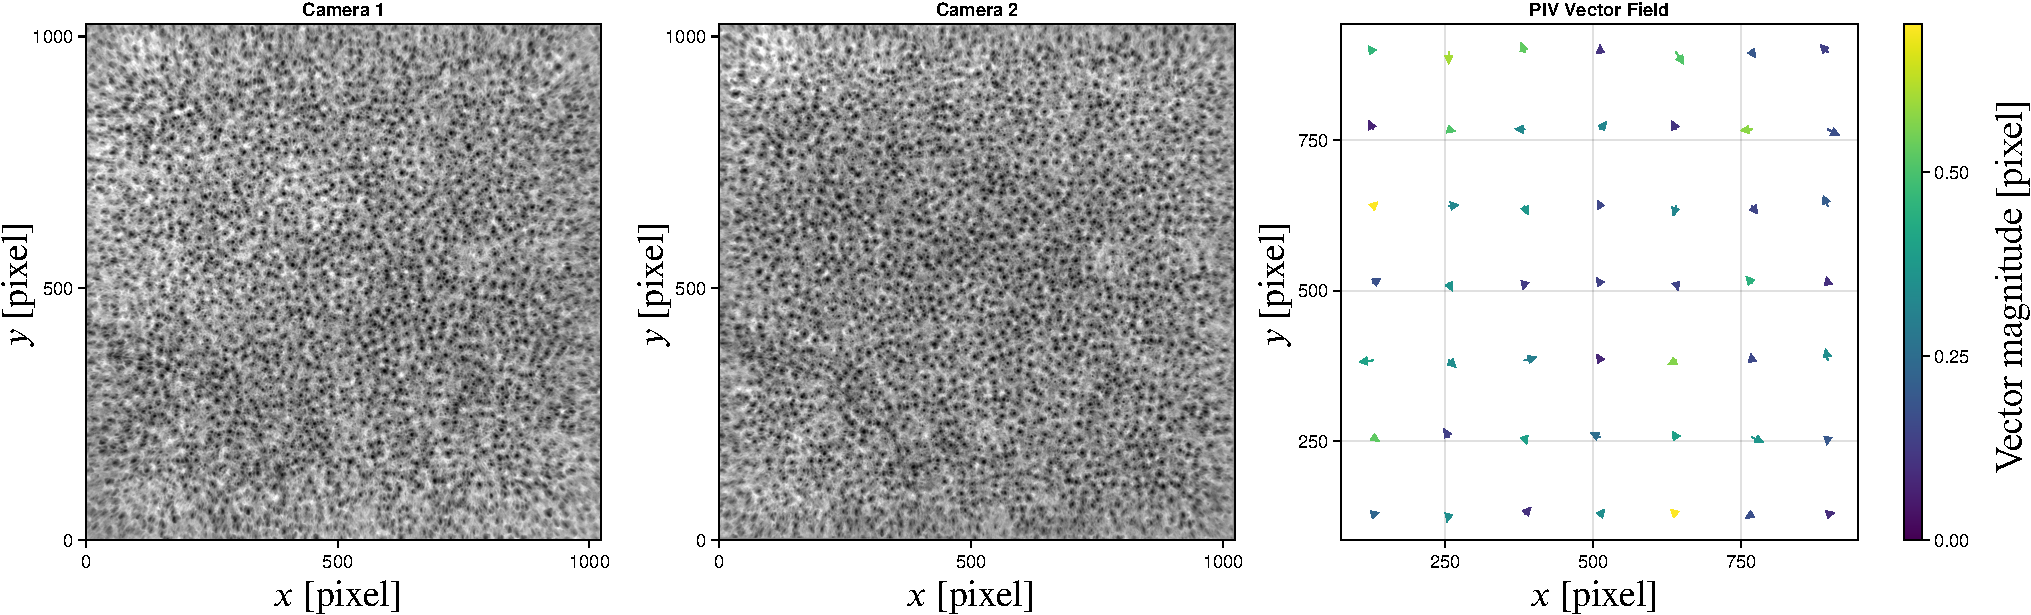
\includegraphics[width=0.98\linewidth]{./Figure/3_Methods/afterbundle.pdf}
    \caption{Reconstructed two random dot images after bundle adjustment. Two images are contrast-enhanced for visualization.}
    \label{fig:afterbundle}
\end{figure}
以上の手続きで2枚の画像を全域で\SI{1}{pixel}以下の誤差で校正できることを確認した.